% !Mode:: "TeX:UTF-8" 

\chapter{\hei \textbf{研究背景}}

%=========================================================================================
\section{\hei 支持向量机基本原理}
\subsection{支持向量机的目的}
支持向量机的理论最初来自数据分类问题。对于数据分类问题,如果采用传统回归机器学习方法来实现,其原理可以简单地描述为算法随机产生一个平面,直到训练集 中属于不同分类的点正好位于平面的不同侧面 。 这种 处 理机 制 决 定 了进行 数 据 分类最 终 获 得的 分 割平面将相 当靠 近 训 练 集 中的点 , 而 在 绝 大多数 情 况下 ,并不是一个最优解 ,同时还增加了训练强度\cite{张松兰2016支持向量机的算法及应用综述}。为此支持向量机考 虑寻 找 一 个 满 足分类要求的分割平面,并使 训 练集 中 的 点距离 该 分割 平 面 尽 可 能地 远 , 即 寻 找 一 个 分 割 平 面 , 使其 两 侧 的空白 区 域 最大,如图\ref{fig:2.1}所示:

\begin{figure}[!h]
	\centering
	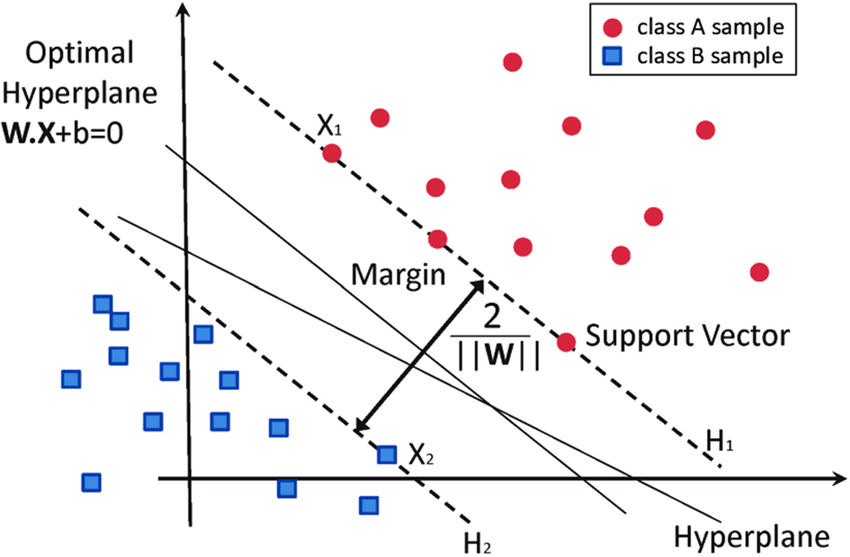
\includegraphics[scale=0.4]{figures/SVM1.png}
	\caption{数据点集实现最大化分类间隔}
	\label{fig:2.1}
\end{figure}
图中红色和蓝色点分别表示两种不同类型的数据,$\omega*x+b=0$、$H_1$、$H_2$是区分两类数据的分割平面。其中 $H_1$,$H_2$是划分两类数据的边缘分割平面,它们之间的距离 margin 就是两类之间的分割间隔,而图中位于分割平面$H_1$,$H_2$上的红色和蓝色点即为支持向量\cite{张松兰2016支持向量机的算法及应用综述}。支持向量机通过先验选择的非线性映射,将输入向量映射到某个高维特征空间$Z$中。在该空间中构造了一个具有特殊性质的线性决策面,保证了数据集的高泛化能力\cite{cortes1995support},其目的就是寻求一个最优的分割平面使两类之间的分割间隔最大。

\subsection{线性两分类支持向量机}
\subsubsection{线性可分两分类}
对于线性可分问题,支持向量机运用优化算法实现最大化分割间隔,即只要一个超平 面$H$就能正确划分所有训练样本的类别。给定训练样本集$(x_i,y_i),i=1,2,...,l,x\in R^n,y\in \{\pm1\}$、,超平面记作$(\boldsymbol{\omega}\cdot \boldsymbol{x})+b=0$ ,为使分类面对所有样本正确分类并且具备分类间隔,就要求它满足如下约束: 
\begin{equation}\label{e1}
    y_i[(\boldsymbol{\omega}\cdot x_i)+b]\ge 1\quad i=1,2,...,l
\end{equation}
可以计算出分类间隔为$\frac{2}{\parallel \omega\parallel}$ ,因此构造最优超平面的问题就转化为在约束式下求:
\begin{equation}\label{e2}
    \min \Phi(\boldsymbol{\omega})=\frac{1}{2}\|\boldsymbol{\omega}\|^{2}=\frac{1}{2}\left(\boldsymbol{\omega}^{\prime} \cdot \boldsymbol{\omega}\right)
\end{equation}
为了实现最优化问题,引入Lagrange函数:
\begin{equation}\label{e3}
    \mathrm{L}(\boldsymbol{\omega}, b, \mathrm{a})=\frac{1}{2}\|\boldsymbol{\omega}\|+a(1-\boldsymbol{y}((\boldsymbol{\omega} \cdot \boldsymbol{x})+b)) 
\end{equation}
\ref{e3}式中,$a_i>0$ 为Lagrange乘数。该QP问题转 化为相应的对偶问题即:
\begin{equation}
\begin{array}{l}
\max Q(a)=\sum_{j=1}^{l} a_{j}-\frac{1}{2} \sum_{i=1}^{l} \sum_{j=1}^{l} a_{i} a_{j} y_{i} y_{j}\left(x_{i} \cdot x_{j}\right) \\ \\
\text { s.t. } \sum_{j=1}^{l} a_{j} y_{j}=0 \quad j=1,2, \cdots, l, a_{j} \geqslant 0, j=1,2, \cdots, l
\end{array}
\end{equation}
解得最优解:$\boldsymbol{a}^{*}=\left(a_{1}^{*}, a_{2}^{*}, \cdots, a_{l}^{*}\right)^{\mathrm{T}}$。
计算最优权值向${\omega}^{*}$和最优偏置${b}^{*}$,分别为:
\begin{equation}\label{e5}
    \begin{array}{c}
\boldsymbol{\omega}^{*}=\sum_{j=1}^{l} a_{j}^{*} y_{j} x_{j} \\ \\
b^{*}=y_{i}-\sum_{j=1}^{l} y_{j} a_{j}^{*}\left(x_{j} \cdot x_{i}\right)
\end{array}
\end{equation}
\ref{e5}式中,下标$j\in \{j|a_{j}^{*}\}$。因此得到最优分类超平面$H$:$(\boldsymbol{\omega^{*}}\cdot \boldsymbol{x})+b_{*}=0$,而最优分类函数为:
\begin{equation}
    \begin{array}{c}
f(\boldsymbol{x})=\operatorname{sgn}\left\{\left(\boldsymbol{\omega}^{*} \cdot \boldsymbol{x}\right)+b^{*}\right\}=
\operatorname{sgn}\left\{\left(\sum_{j=1}^{l} a_{j}^{*} y_{j}\left(x_{j} \cdot x_{i}\right)\right)+b^{*}\right\}, \boldsymbol{x} \in R^{n}
\end{array}
\end{equation}
\subsubsection{线性不可分两分类}
对于训练样本是线性不可分的情况,存在个别训练样本无法满足式\ref{e1}。此时,支持向量机应当允许一定的分类错误。具体的做法是,在式\ref{e1}的约束条件中,引入松弛变量以软化约束条件,同时在目标函数中对松弛变量进行惩罚以避免松弛变量取值过大而引起的大量错分情况\cite{胡春2018支持向量机研究综述}。也就是说,线性不可分两类分类支持向量机求解下列问题:
\begin{equation}
\begin{aligned}
& \min _{\omega, b, \xi_t} \Phi(\boldsymbol{\omega})+C \sum_t \xi_t, \\
& \text { s.t. }\left\{\begin{array}{c}
(\omega)^T x_i+b \geq 1-\xi_t, \text { if } a_t=+1, \\
(\omega)^T x_i+b \leq-1+\xi_t, \text { if } a_t=-1, \\
\xi_t \geq 0 .
\end{array}\right. \\
&
\end{aligned}
\end{equation}

\subsection{非线性两分类支持向量机}
客观世界大多都是非线性的训练样本,尤其是不可分问题,对于非线性不可分问题,支持向量机通过适当的核函数将输入空间映射到高维空间,将非线性问题转化线性问题,实现高维空间线性可分,然后在新空间中利用二次型寻优算法求取最优线性分类面,从而将两类样本区分开来\cite{sebald2000support,萧嵘2000支持向量机理论综述}。

在上面的对偶问题中, 都只涉及训练样本之间的内积运算,这样,在高维空间实际上只需进行内积运算,而这种内积运算是可以用原空间中的函数实现的,我们甚至没有必要知道变换的形式\cite{张学工2000关于统计学习理论与支持向量机}。根据泛函的有关理论,只要一种核函数$K(x_i,x_j)$满足$Mercer$条件,它就对应某一变换空间中的内积\cite{vapnik1999nature}。

因此, 在最优分类面中采用适当的内积函数$K(x_i,x_j)$就可以实现某一非线性变换后 的线性分类, 而计算复杂度却没有增加\cite{张学工2000关于统计学习理论与支持向量机}, 此时约束条件\ref{e3}变为:
\begin{equation}
\Phi(\boldsymbol{\omega})=\sum_{i=1}^n \alpha_i-\frac{1}{2} \sum_{i, j=1}^n \alpha_1 \alpha_j y_i y_j K\left(x_i, x_j\right)
\end{equation}


{\hei 支持向量机的核心是选择合适的核函数和参数,它们直接影响了模型的预测能力和泛化能力。为了解决不同的问题,我们需要根据数据特征和目标函数来选择最优的核函数和参数。然而,这是一个具有挑战性的问题,因为我们需要在速度和准确性之间找到最佳的折中。}

下面,给出求解非线性两分类问题的支持向量机算法一般框架如下:

\begin{algorithm}[H]	
	\floatname{algorithm}{算法}
	\caption{(支持向量机算法)}
	\renewcommand{\algorithmicrequire}{\textbf{输入:}} 
	\renewcommand{\algorithmicensure}{\textbf{输出:}}
	
	\begin{algorithmic}[1]
		\State  准备数据,将数据分为训练集和测试集,确定特征和标签
		\State 选择核函数,根据数据的分布和复杂度选择合适的核函数
		\State  训练模型,找到最优的超平面,并确定支持向量和分类边界
		\State  预测数据,将测试集输入模型,根据超平面的位置判断并计算准确率和误差
		\State  评估结果,根据预测的效果和目标,调整参数或核函数,优化模型的性能
	\end{algorithmic}
\end{algorithm}	

